\documentclass{article}
\usepackage{graphicx} % Required for inserting images
\usepackage[margin=2cm, top=3cm]{geometry} % margine superiore ridotto a 1 cm
\usepackage{listings}
\usepackage{subcaption}  % Pacchetto per sottodidascalie
\usepackage{float}       % Pacchetto per posizionamento rigido delle figure


\begin{document}



\section{Reti di raccolta e reti di accesso}
\subsection{Introduzione alle reti di raccolta e di accesso}
Abbiamo introdotto i concetti di: \\\\
\textbf{LAN}: trasmissione tra due stazioni in una topologia complessa, con ap, bridge e repeater\\\\
\textbf{WAN}: trasmissione tra due stazioni su un canale punto-punto\\\\
Tra di loro vi è una zona intermedia costituita da una rete di raccolta e una rete di accesso.
\subsection{Rete di raccolta}
\begin{figure}[h]
    \centering
    \begin{minipage}{0.4\textwidth} % Imposta la larghezza della colonna sinistra
        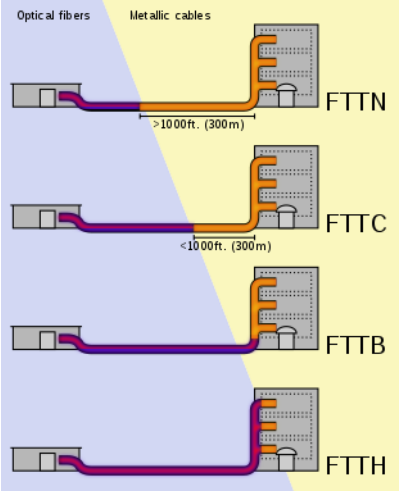
\includegraphics[width=6cm,height=6cm]{immagine_2024-11-05_165254252.png}
        \caption{Reti di raccolta del traffico} % Opzionale
        \label{fig:immagine}
    \end{minipage}%
    \hfill
    \begin{minipage}{0.55\textwidth} % Imposta la larghezza della colonna destra
        \textbf{FTTN (Fiber To The Node)} e \textbf{FTTC (Fiber To The Cabinet)} sono i metodi di raccolta più comuni e corrispondono alle tecnologie conosciute come xDSL (xDigital Subscriber Line) (al posto della x possono esserci varie lettere a seconda di alcuni parametri come la banda) \\
        \textbf{FTTB (Fiber To The Building)} e \textbf{FTTH (Fiber To The Home)} sono i metodi di raccolta in corso di realizzazione e sono in grado di garantire linee a più di 1Gbit/sec; fanno uso di OLT (GPON)
    \end{minipage}
\end{figure}

\vspace{1pt} % Aggiunge uno spazio verticale tra le due sezioni (opzionale)
\noindent %Per togliere lo spazietto fastidioso
\begin{figure}[H] 
    \centering
    \vspace{-55pt} % Riduce lo spazio sopra l'immagine
    \begin{minipage}{0.4\textwidth} % Colonna per le immagini
        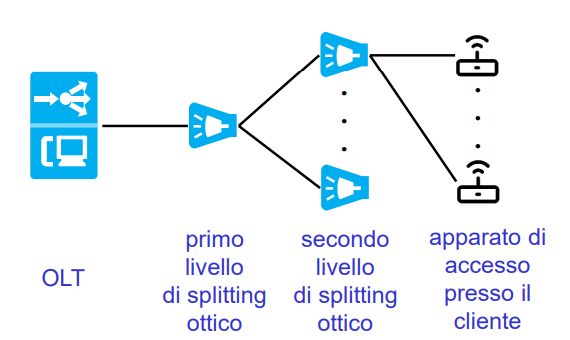
\includegraphics[width=7cm, height=4cm]{Screenshot 2024-11-05 165935.png} % Prima immagine
        \vspace{10pt} % Spazio verticale tra le immagini
        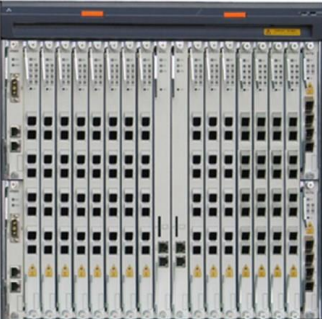
\includegraphics[width=6cm, height=5cm]{Screenshot 2024-11-05 165947.png} % Seconda immagine
        \caption{Optical Line Termination} % Opzionale
    \end{minipage}%
    \hfill
    \begin{minipage}{0.55\textwidth} % Colonna per il testo
       \textbf{GPON (Gigabit-capable Passive Optical Network)} è una tecnologia per la raccolta del traffico dei clienti, fa uso di apparati chiamati OLT (Optical Line Termination), sui quali arrivano le fibre ottiche dei clienti, un OLT è essenzialmente uno switch in cui su ogni porta possono essere collegati fino a 64 clienti. Nello splitting ottico i dispositivi non devono essere alimentati da corrente ma mettono assieme dati di diversi clienti.
        
        \vspace{20pt} % Spazio verticale tra i blocchi di testo
    \end{minipage}
\end{figure}
\noindent
\subsection{La rete di accesso}
Tra la rete di raccolta e la WAN c'è la rete di accesso. È una rete di switch con un'estensione geografica significativa, tuttavia non può essere troppo grande perchè vogliamo evitare che ci siano switch a cascata uno dentro l'altro, viene anche chiamata \textbf{MAN (Metro Area Network)}.\\
Per rispondere ai requisiti prestazionali e di manutenibilità l'architettura è molto semplice. Ed è composta da switch connessi in un anello, questo risulta utile per la ridondanza, infatti, in caso si rompa qualcosa la rete continuerebbe a funzionare. Gli switch non restano accesi tutti contemporaneamente ma resta acceso soltanto lo spanning tree.
\subsection{Architettura delle reti di accesso}
\begin{figure}[h]
    \centering
    \begin{minipage}{0.4\textwidth} % Imposta la larghezza della colonna sinistra
        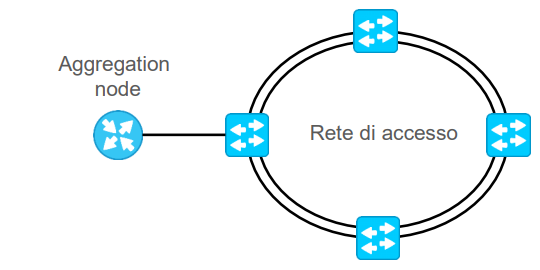
\includegraphics[width=7cm,height=4cm]{immagine_2024-11-05_171121175.png}
        \caption{Architettura delle reti di accesso} % Opzionale
        \label{fig:immagine}
    \end{minipage}%
    \hfill
    \begin{minipage}{0.55\textwidth} % Imposta la larghezza della colonna destra
        Un \textbf{aggregation node} collega la rete di accesso al backbone (WAN) del provider. Se si rompe uno switch, solo i clienti attestati su quello switch hanno un disservizio. Per aumentare la robustezza dell'anello spesso si realizzano doppi collegamenti.
    \end{minipage}
\end{figure}
\section{Metodi e modelli per il livello di rete}
\subsection{Il livello di rete}
Il livello di rete sceglie una strada per i pacchetti, la strada verso la destinazione è composta da vari passaggi intermedi (salti o hop).\\
In rosso la strada stabilita dal livello 3 per la comunicazione
\begin{figure}[H] % Usa 'H' per forzare la posizione qui
    \centering % Centra l'immagine
    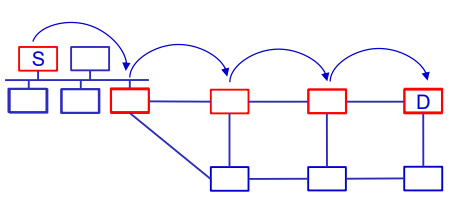
\includegraphics[width=7cm, height=4cm]{immagine_2024-11-05_172108640.png} % Percorso dell'immagine
    \label{fig:immagine} % Etichetta per riferimento
\end{figure}
\noindent
Il livello di rete fornisce servizi al livello di trasporto, il quale non è interessato a conoscere: il numero e la topologia delle varie reti, che vengono attraversate per raggiungere una destinazione e le tecnologie di livello inferiore usate per realizzare le reti attraversate. I servizi offerti dal livello di rete al livello di trasporto possono essere connessi (il che prevede un dialogo tra dispositivi con dei riscontri) o non connessi. L'instradamento può essere a datagramma o a circuito virtuale. Un livello di rete connesso fa tipicamente uso della commutazione a circuito virtuale mentre uno non connesso fa uno della commutazione a datagramma.\\
\vspace{-91pt}
\begin{figure}[H]
    \centering
    \begin{minipage}{0.55\textwidth} % Imposta la larghezza della colonna sinistra
        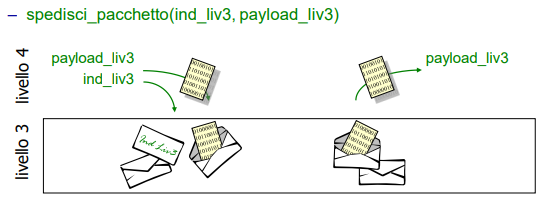
\includegraphics[width=9cm,height=4cm]{Screenshot 2024-11-05 174356.png}
        \caption{Interfaccia con il livello 4} % Opzionale
        \label{fig:immagine}
    \end{minipage}%
    \hfill
    \begin{minipage}{0.45\textwidth} % Imposta la larghezza della colonna destra
        Il livello di trasporto (livello 4) ha bisogno di conoscere le macchine attraverso indirizzi univoci, distribuiti in modo consistente su tutta la rete. Nell'immagine vi è un esempio di primitiva di servizio (una funzione) non connesso offerta al livello di trasporto. Ind rappresenta l'indirizzo del destinatario, mentre Payload il contenuto del pacchetto.
    \end{minipage}
\end{figure}
\noindent
Dal punto di vista del livello 3 i sistemi sulla rete possono essere: \textbf{End System (es)} o \textbf{Intermediate System (is)}. A ogni sistema viene associato un indirizzo numerico e un nome, informazioni sulla corrispondenza nomi-indirizzi sono gestite da server appositi, chiamati name server.
Gli is, chiamati anche router o gateway, operano a livello 3 e contengono gli strati 1, 2 e 3 dell'architettura iso-osi. Vi è bisogno di trovare un modo per far corrispondere gli indirizzi di livello 2 (MAC) con gli indirizzi di livello 3 (identificatore nell'intera rete).
\subsection{Metodi di instradamento}
Gli is possono effettuare instradamento con tre metodi principali:\\\\
\textbf{Routing by network address}
\begin{figure}[H]
    \centering
    \begin{minipage}{0.55\textwidth} % Imposta la larghezza della colonna sinistra
        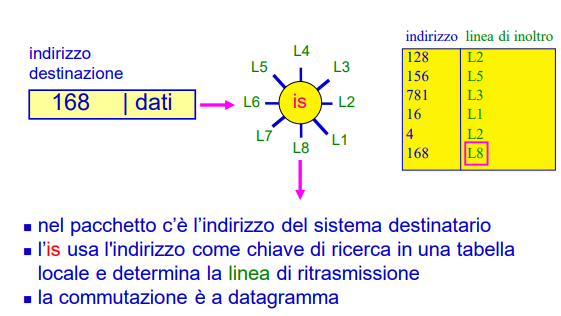
\includegraphics[width=9cm,height=5cm]{immagine_2024-11-05_175738613.png}
        \caption{Routing by network address} % Opzionale
        \label{fig:immagine}
    \end{minipage}%
    \hfill
    \begin{minipage}{0.45\textwidth} % Imposta la larghezza della colonna destra
        Questo metodo è valido indipendentemente da chi compila la tabella. Se l'indirizzo non fosse presente nella tabella il pacchetto verrebbe buttato, al contrario di uno switch che l avrebbe mandato a tutti. La tabella di un is che fa routing by network address contiene l'elenco di tutti gli indirizzi presenti nella rete.
    \end{minipage}
\end{figure}
\noindent
\textbf{Label (senza) swapping}
\begin{figure}[H]
    \centering
    \begin{minipage}{0.55\textwidth} % Imposta la larghezza della colonna sinistra
        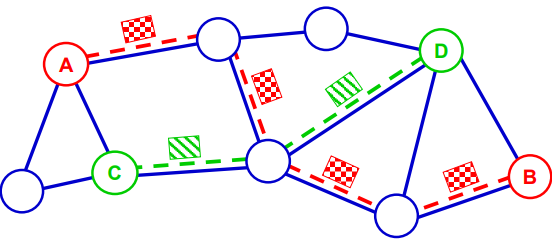
\includegraphics[width=9cm,height=5cm]{immagine_2024-11-05_180243944.png}
        \caption{Label (senza) swapping} % Opzionale
        \label{fig:immagine}
    \end{minipage}%
    \hfill
    \begin{minipage}{0.45\textwidth} % Imposta la larghezza della colonna destra
       La commutazione è a circuito virtuale. Nel pacchetto c'è un eticchetta che identifica il circuito virtuale. Ogni is usa la label come chiave di ricerca in una tabella locale, molto piccola, e determina la linea di ritrasmissione. Quello che notiamo è che i pacchetti vengono colorati e avranno un colore che identifica il percorso, questo serve a far capire agli is dove mandare il pacchetto. La tabella di un is che fa label swapping contiene l'elenco dei circuiti virtuali che lo attraversano in un certo istante.
    \end{minipage}
\end{figure}
\noindent
\textbf{Label swapping}
\begin{figure}[H]
    \centering
    \begin{minipage}{0.55\textwidth} % Imposta la larghezza della colonna sinistra
        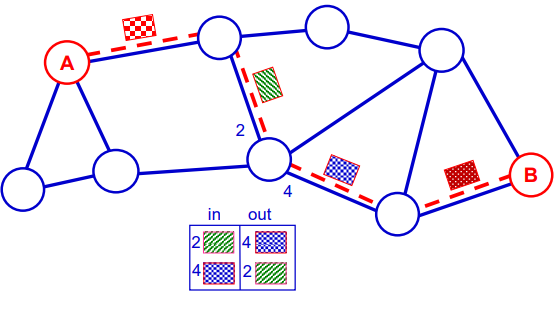
\includegraphics[width=9cm,height=5cm]{immagine_2024-11-05_181233773.png}
        \caption{Label swapping} % Opzionale
        \label{fig:immagine}
    \end{minipage}%
    \hfill
    \begin{minipage}{0.45\textwidth} % Imposta la larghezza della colonna destra
      Per evitare di dover verificare nell'intera rete che una specifica label non sia già utilizzata per qualche altra connessione, ad ogni tratto del circuito è assegnata una label (in generale) diversa ed assegnata localmente. In questo modo la label può essere scelta localmente dagli is che condividono il link
    \end{minipage}
\end{figure}
\noindent
\textbf{Source Routing}
\begin{figure}[H]
    \centering
    \begin{minipage}{0.55\textwidth} % Imposta la larghezza della colonna sinistra
        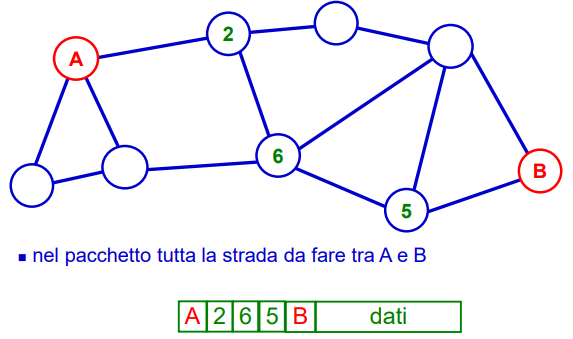
\includegraphics[width=9cm,height=5cm]{immagine_2024-11-05_181446921.png}
        \caption{Source Routing} % Opzionale
        \label{fig:immagine}
    \end{minipage}%
    \hfill
    \begin{minipage}{0.45\textwidth} % Imposta la larghezza della colonna destra 
    \end{minipage}
\end{figure}
\noindent
Un router fa sostanzialmente due funzioni: Control Plane. Data Plane, arriva un pacchetto, guarda la tabella di instramento e fa un azione sul pacchetto
\begin{figure}[H] % Usa 'H' per forzare la posizione qui
    \centering % Centra l'immagine
    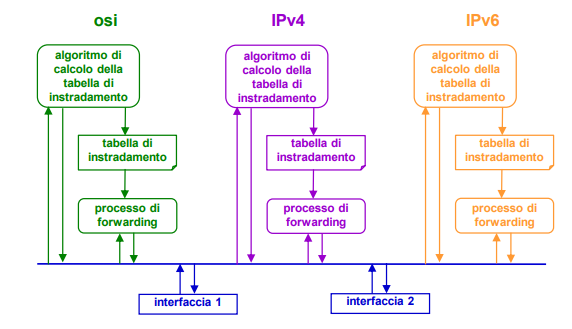
\includegraphics[width=10cm, height=6cm]{immagine_2024-11-05_181851825.png} % Percorso dell'immagine
    \label{fig:immagine} % Etichetta per riferimento
\end{figure}
\noindent
\section{IPv4, ARP e la suite TCP/IP}
\subsection{Introduzione}
Il protocollo IPv4 (Internet Protocol versione 4) è il principale protocollo di rete (di livello 3) della "suite TCP/IP", detta anche "Internet Protocol Suite". La suite TCP/IP è la pila protocollare usata in Internet ed è implementata nella stragrande maggioranza dei computer. I protocolli della suite sono descritti da documenti chiamati Request For Comments (RFC).
\subsection{IPv4}
È attualmente, assieme a IPv6, il protocollo principale di lvl. 3. È provvisto di funzioni di instradamento, frammentazione, riassemblaggio e rilevazione di errori. Riceve messaggi dai protocolli UDP e TCP del livello superiore. I suoi pacchetti vengono detti IPv4 datagram. La dimensione del datagram dipende dai vincoli del livello 2. Se il datagram è troppo grande, IPv4 provvede alla frammentazione.  Provvedere al routing è semplice nel caso in cui il datagram viaggi all'interno di una LAN, più complesso se la spedizione coinvolge un computer remoto. Lo strato IPv4 di un router non può comunque riassemblare i datagrammi.
\subsubsection{IPv4 datagram}
Analogamente ai pacchetti di livello 2, il datagram IPv4 è diviso in due parti: \textbf{l'header e i dati}. L'header contiene gli indirizzi del mittente e del destinatario.
\begin{figure}[H] % Usa 'H' per forzare la posizione qui
    \centering % Centra l'immagine
    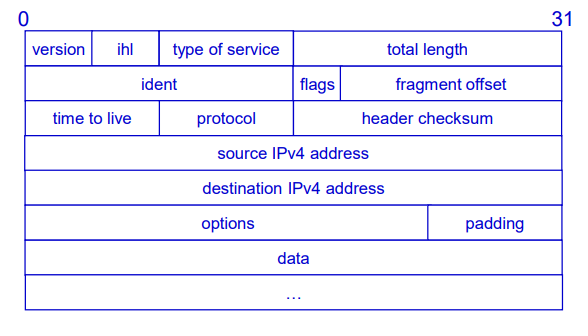
\includegraphics[width=10cm, height=6cm]{immagine_2024-11-07_141921833.png} % Percorso dell'immagine
    \label{fig:immagine} % Etichetta per riferimento
\end{figure}
\noindent
\textbf{Version}: è il numero di versione del protocollo IP che ha generato il pacchetto, attualmente vale 4. Grazie al campo version la migrazione tra due versioni può essere più chiara, lenta e controllata.\\
\textbf{IHL (Internet Header Length)}: è la lunghezza dell'header espressa in parole da 32 bit (4byte), il valore minimo è 5.\\
\textbf{Type of service}: Il campo type of service specifica la priorità di un datagram rispetto a un altro.\\
\textbf{I campi ident, flags e fragment offset}: Ci aiutano nella frammentazione di un pacchetto, ma perchè frammentare un pacchetto?
Ogni livello due attraversato potrebbe avere una maximum transmission unit (MTU dimensione massima di un pacchetto) diversa, il pacchetto di livello tra potrebbe essere troppo grande per essere imbustato in un data link intermedio
\begin{figure}[H] % Usa 'H' per forzare la posizione qui
    \centering % Centra l'immagine
    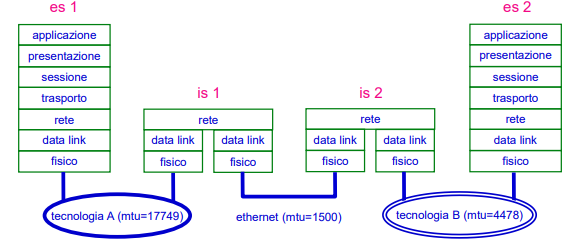
\includegraphics[width=13cm, height=3cm]{Screenshot 2024-11-07 142627.png} % Percorso dell'immagine
    \label{fig:immagine} % Etichetta per riferimento
\end{figure}
\noindent
Mettiamo caso che arrivi un pacchetto da sinistra da 17749 (MTU) l'is sarà costretto a frammentare in pacchetti da 1500 (MTU), il secondo is invece ha una tecnologia che ha MTU 4478 nonostante ciò non può riassemblare il pacchetto.\\
Per frammentare intendiamo la suddivisione di un pacchetto in pacchetti più piccoli, il riassemblaggio del pacchetto originale viene fatto invece sulla macchina di destinazione. Ovviamente occorrono degli appositi campi nell header di livello tre che consentano di: riconoscere il pacchetto come frammento, riconoscere i frammenti generati dallo stesso pacchetto e determinare l'ordine dei frammenti in maniera da poter riassemblare il pacchetto originale. L'adozione di un semplice contatore non rende possibile la frammentazione di un pacchetto già frammentato. Per questo si utilizza un offset che ci permette di riframmentare un pacchetto già frammentato.\\\\
\textbf{Ident}: intero che identifica un datagramma, serve all’IPv4 dell’host ricevente nel momento del riassemblaggio; due datagrammi con lo stesso ident vengono riassemblati nello stesso pacchetto.\\
\textbf{Fragment Offset}: serve a riunire i frammenti nel giusto ordine, può specificare solo un offset multiplo di 8. Tutti i frammenti eccetto l'ultimo hanno un numero di byte multiplo di 8.\\
\textbf{Flags}: Il primo bit è riservato e deve essere sempre 0. DF (Don't fragment) specifica se il datagram può essere frammentato. MF (more fragment) permette di riconoscere l'ultimo frammento del pacchetto.
\begin{figure}[H] % Usa 'H' per forzare la posizione qui
    \centering % Centra l'immagine
    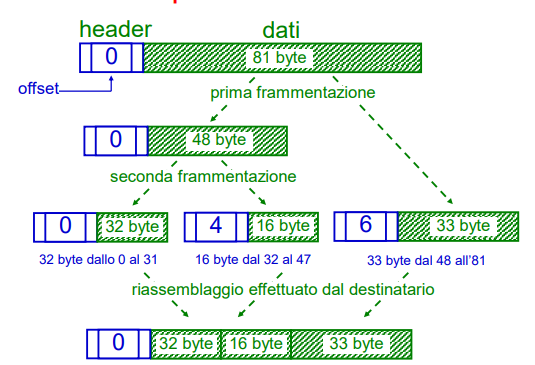
\includegraphics[width=12cm, height=7cm]{immagine_2024-11-07_161036682.png} % Percorso dell'immagine
    \label{fig:immagine} % Etichetta per riferimento
\end{figure}
\noindent
I numeri dell offset vanno sempre moltiplicati per 8. Es. 6x8=48 quindi il frammento parte dal byte 48.\\\\
\textbf{Total Length}: è la lunghezza del pacchetto completo di header e payload.
\textbf{Time to Live}: Specifica qual'è il tempo di vita del pacchetto, viene decrementato col passare del tempo, in particolare a ogni "hop" (salto) , quando vale 0 il pacchetto viene scartato. Quando il pacchetto è scartato il router manda un avvertimento al mittente.\\
\textbf{Protocol}: identifica il protocollo di livello superiore che è nel payload del pacchetto IPv4.\\
\textbf{Header Checksum}: riguarda solo l'header, deve essere ricalcolato a ogni hop.\\
\textbf{Options}: Viene utilizzato per informazioni meno frequenti nei pacchetti e per sperimentazione; Ogni opzione inizia con 1 byte di codice che ne specifica il tipo.
\end{document}
